\chapter{LEVINSON'S THEOREM Problem of Continuation}\label{chap12}%Lect 12

\section[Levinson's theorem on entire functions...]{Levinson's theorem on entire functions of exponential type
 and its application to the problem of closure}\label{chap12:sec1}%Sec 1 

\noindent
\textbf{Levinson's theorem}\pageoriginale \textit{Let $ \Phi (w)$ be an entire
 function of exponential type, having $(-ik, ik)$ as its conjugate
 diagram and satisfying the following condition} 
\begin{equation}
 \int^\infty_1 \log | \Phi (u)\Phi (-u) | \frac{du}{u^2} < \infty \tag{a}
\end{equation}
\textit{Let $r_k e^{i \theta_ k}$ be the zeros of $\Phi (w)$ with
 $N_r(r)$ the distribution of zeros of $\Phi(w)$ in the right half -
 plane and $N_\ell (r)$ the distribution of zeros of $\Phi(w)$ in the
 left half-plane. Under these conditions, the following relations
 hold:} 
\begin{align*}
 \sum \left\{ | \sin \theta_k| / r_k \right\} & < \infty
 \tag{1}\label{chap12:sec1:eq1} \\
 \lim_{r \rightarrow \infty } \frac{N_r(r)}{r} &= D = \lim_{r
 \rightarrow \infty} \frac{N_\ell (r)}{r}, D = k/\pi
 \tag{2}\label{chap12:sec1:eq2}  
\end{align*}

The first part is proved by applying Carleman's formula, but the
second part is more involved. (Levinson, Chap. $III$). 

Let us consider the problem of closure of $\{e^{i \lambda x}
\}_{\lambda \in \Lambda}$ in an interval $I$ if length $|I|$. We want
to find conditions on $|I|$ and in order that $\{e^{i \lambda x}
\}_{\lambda \in \Lambda}$ be total in $\mathscr{C}(I)$; in other
words, we want to find conditions on $|I|$ and $\Lambda$ in order that
the following relation holds; $\{ \Phi (w)$ is an entire function of
exponential type $\le \dfrac{|I|}{2}$ with $\Phi(u)$ bounded and $\Phi
(\Lambda) = 0 \} \Rightarrow \Phi \equiv 0$. We have already studied this
problem by means of Jensen's and Carleman's formulae. In order to find
new conditions on $\Lambda$ we first define the \textit{ maximum
 density } of Polya. 

\begin{defi*}
 Given\pageoriginale a sequence $\Lambda$, consider sequences $\Lambda'$ having
 density $D'$ and $\Lambda' \supset \Lambda$. If the set of $\Lambda'$
 is empty we define the maximum density, $D_{Max}$, of $\Lambda$ to
 be $\infty$. Otherwise, $D_{Max} = \inf\limits_{\Lambda' \supset
 \Lambda}$ (density $D'$ of $\Lambda'$) 
\end{defi*}

Now the zeros of $\Phi$ form a sequence $\Lambda' \supset
\Lambda$. Denoting by $\Lambda^+ and \Lambda^-$ the set of $\lambda
\in \Lambda$ in the right half plane and left half plane respectively,
we have by Levinson's theorem that $\Lambda'^{+} and \Lambda'^{-}$ have the
same density $D, D \ge D_{Max}$ of $\Lambda^+$ and $D \ge D_{Max}$ of
$\Lambda^-$. Moreover, $D = \dfrac{k}{\pi}, k$ being the type of
$\Phi$. Thus we have the following closure theorem: 

\begin{theorem*}[(Levison)]
 $$
 \{ |I| < 2 \pi D_{Max} \text{ of }\Lambda^+ \}\text{ or }\{ |I| <
 2 \pi D_{Max}\text{ of } \Lambda^- \} \Rightarrow
 \mathscr{C}_{\lambda}(I) = \mathscr{C} (I). 
 $$
\end{theorem*}

We have a similar theorem for the spaces $\mathscr{D}(I) or
\mathscr{E}$. Theorems of this type apply to sequences which do not
have a density. For example, take the sequence formed of 
$$
\{ 10^N, 10^N + 1, 10^N + 2, \ldots, 10^N + 10^{N-1} \} \text{ for }
N = 10^{10^n}, n= 1, 2, \ldots 
$$
It has $D_{Max} = 1$ but has no density and even the upper density is
very small $(D = \dfrac{1}{11})$. One can easily calculate the
maximum density of Polya by the following formula: 
$$
D_{Max}~ \text{of}~ \Lambda = \limsup_{k \nearrow 1} \left[ \limsup_{r
 \rightarrow \infty} \left\{\frac{n(kr) - n(r)}{kr - r} \right\}\right] 
$$
We shall give a proof of this result in appendix $I$.

The above theorem of closure gives immediately that the mean period of
a mean periodic function $f, L \ge 2 \pi D_{Max}~\text{ of }~\Lambda^+$ and $L
\ge 2 \pi\break D_{Max} ~\text{of}~ \Lambda^-$ where $\Lambda$ is the spectrum of
$f$. 

The\pageoriginale theorem about the supports of the convolution of two distributions
can be deduced from Levinson's theorem as follows: 

If $T$ is a distribution with segment of support $I$, the density of
zeros of its Fourier transform $\mathscr{C}(I)$ (either in Re $z > 0$
or Re $z < 0)$ is $|I| /2 \pi$. It is sufficient to show this when $I
= [-k, k]$: then $\mathscr{C}(T)$ satisfies the hypothesis of
Levinson's theorem. 

\begin{theorem*}[on supports] 
  $T = T_1 * T_2 \Rightarrow I = I_1 + I_2$.
\end{theorem*}

Since we know that $I \subset I_1 + I_2 $, it is sufficient to show
that $|I| = |I_1| + |I_2|$. This results from the fact that the density
of zeros of $\mathscr{C}(T) = \mathscr{C}(T_1) \mathscr{C}(T_2)$ is
the sum of the density of zeros of $\mathscr{C}(T_1)$ and that of
$\mathscr{C}(T_2)$. 
 
We shall see another application of Levinson's theorem, to a problem
of quasi - analyticity, in lecture \ref{chap19}. 
 
\section[Problem of continuation - Description of the
  problem]{Problem of continuation - Description of the\hfil\break
  problem}\label{chap12:sec2}%Sec 2 
 
Consider a function $f \in \mathscr{H}_{\Lambda}(\Omega)$ (or
$\mathscr{C}_{\Lambda}(I), \mathscr{D}'(I)$ etc. We suppose
$\mathscr{H}_{\Lambda}(\Omega) \neq \mathscr{H}(\Omega)~
(\mathscr{C}_{\Lambda}(I) \neq \mathscr{C}(I) etc)$. Then the natural
question is to ask whether one can continue it beyond $\Omega(or
I)$. More precisely, we have to give conditions on $\Lambda$ and
$\Omega$ so that every $f \in \mathscr{H}_{\Lambda}(\Omega)$ (or
$\mathscr{C}_{\Lambda}(I)$ etc.) is analytically continuable into a
domain $G \supset \Omega $(or into $R$); then we have to give
properties of $f$ in $G(or R)$ in terms of its properties in $\Omega
(or I)$ (See foot note $p. 71 @$) 
 
\noindent 
\begin{minipage}[c]{5.8cm}
 \quad First, let $\Omega_0$ be an open set, $\Omega_\zeta$ the translate of
$\Omega$ by the translation carrying $0$ into $\zeta$; suppose $f \in
\mathscr{H}_{\Lambda}(\Omega_o) \neq \mathscr{H}(\Omega_o)$, and $f$ is
analytically continuable into a domain generated by a chain of
translates of $\Omega_0$. i.e., $f \in \mathscr{H}(\Omega_{\zeta})$,
for every $\zeta$ belonging to a curve $C$ with origin in $O$. 
\end{minipage}
\begin{minipage}[c]{5cm}
\begin{figure}[H]
\centerline{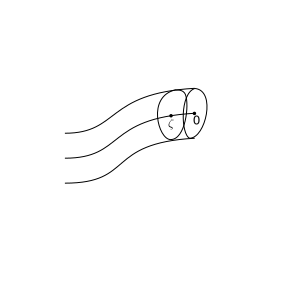
\includegraphics{vol15-figures/fig15-4.eps}}
\end{figure}
\end{minipage}

We\pageoriginale shall
show that $f \in \mathscr{H}_{\Lambda}(\Omega)$. For this, it is
sufficient to prove that if $\int_{\Omega} e^{\lambda z} d\mu (z) =0$
for every $\lambda \in \Lambda$ and if we set 
 $$
 g(\zeta) = \int\limits_{K \subset \Omega} f(z - \zeta) d \mu (z),
 \zeta \in C, 
 $$
 then $g(\zeta) \equiv 0$. But $g (\zeta)$ is analytic in a
 neighbourhood of $C$ and zero in a neighbourhood of 0. So $g(\zeta)
 \equiv 0$. 
 
\noindent 
\begin{minipage}[c]{5.8cm}
\quad Suppose now $\Omega$ is the right half plane. $\Omega = \{u \ge 0
 \}$. Let $f \in \mathscr{H}_{\Lambda}(\Omega) \neq
 \mathscr{H}(\Omega)$. For example, $f$ can be a Dirichlet series $f =
 \sum a (\lambda) e^{\lambda z} ( \lambda$ negative). In any case $f
 \sim \sum a (\lambda) e^{\lambda z}$. Let $G$ be the domain formed by
 the right half-plane and parallel strips projecting into the left
 half- plane. (see figure ). 
\end{minipage}
\begin{minipage}[c]{5cm}
\begin{figure}[H]
\centerline{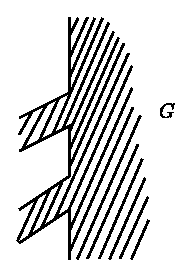
\includegraphics{vol15-figures/fig15-5.eps}}
\end{figure}
\end{minipage}
\medskip

Suppose $f \in \mathscr{H}(G)$, i.e., $f$
 is continuable in $G$. Every bounded subset of $G$ can be translated
 in $G$ until it is in $\Omega$. Then, if $d \mu$ is a measure with
 compact support in $G$, orthogonal to $\{e^{\lambda z} \}_{\lambda
 \in \Lambda}$, its support is in $\Omega_z$ which can be related to
 an $\Omega_o \subset \Omega$ by a chain of translates $\subset
 G$. Under these conditions, we have just seen that $f \in
 \mathscr{H}_{\Lambda}(\Omega_o)$ and $f \in \mathscr{H}(G)
 \Rightarrow f \in \mathscr{H}_{\Lambda}(\Omega_{\zeta})$, i.e., $f$
 orthogonal to $d \mu $. Then, $f \in \mathscr{H}_{\Lambda}(G)$. This
 proves the existence of a sequence $\sum \limits^N_{o} a_N (\lambda)
 e^{\lambda z} \rightarrow f ~\text{in}~ \mathscr{H}(G)$. In the case of
 Dirichlet series, when $\Omega$ is the half-plane of convergence,
 this is called ultra convergence. By means of a conformal mapping, we
 get a result about ultra convergence of Taylor's series;
 corresponding to the case when the strips in $G$ are horizontal, we
 obtain a classical result about ultra convergence in a star domain
 (that is usually obtained by the method of Mittag Leffler, which
 gives a summation process). 
 
 We\pageoriginale now give an analogous result on the line.
 
\begin{defi*}%def
 A class $K \{ M_n\}$ of $C^{\infty}$ functions on the line is
 defined to be the class of $f$ satisfying the condition that $f \in
 K \{ M_n \}$ if and only if for every $n, |f^{(n)} (x)| < k M_n $ on a
 closed interval $J, k$ being constant $k(J)$ depending on $J$ and
 $f$; 
 \end{defi*} 
2. $K \{M_n \}$ is said to be quasi - analytic if the only function
of the class all of whose derivatives vanish at the origin is the zero
function (see lecture 19, \S \ref{chap19:sec1}). 

Suppose further $f$ can be continued on the line in such a manner that
$f \in K\{ M_n\}$. Then $f$ is mean periodic with spectrum
$\Lambda$. For let $d \mu$ be a measure with $\int e^{i \lambda x}
d\mu(x) = 0$ for every $\lambda \in \Lambda$. Let $g (\xi) = \int_I
f(x + \xi) d\mu (x)$, where $I$ is the support of $d \mu$. Now $f \in
K \{ M_n\} \Rightarrow g \in K \{ M_n\}$. But $g^{(n)} (0) = 0$ for
all $n$. So $g = 0$. This means that $f$ and all its translates are
orthogonal to $d \mu$, i.e., $\tau (f) \neq \mathscr{C}$. This gives
that if $f \in \mathscr{C}_\lambda (I)$ and $f \in \mathscr{C}(R)$, in
order that $f \in \mathscr{C}_{\Lambda}(R)$ it is sufficient that $f
\in K \{ M_n\}$ quasi - analytic. This kind of result was first given
by $S$. Mandelbrojt (Mandelbrojt 1). 

\noindent
$@$ These problems are considered in the lectures \ref{chap13},
\ref{chap15} and \ref{chap16}
for the complex plane, and in the lectures \ref{chap17} and \ref{chap18} for the
line. We give now some very easy results. 
